
\chapter{Integración}

En este capítulo vamos a estudiar el concepto que, junto con el de derivada, forma el núcleo del cálculo diferencial e integral.
Veremos que dicho concepto, el de \emph{integral}, será definido por motivos totalmente ajenos a los que nos llevaron a definir la derivada, pero también veremos que está íntimamente conectado a través del teorema fundamental del cálculo.

\section{La integral definida de una función continua}
% Seguimos el Salas-Hille

La noción de integral definida como la presentaremos aquí aparece naturalmente cuando se intenta resolver el problema del cálculo del área de una región plana. El lector recordará la fórmula del área de ciertas figuras planas, por ejemplo el rectángulo el triángulo, el círculo, etc.

\centerline{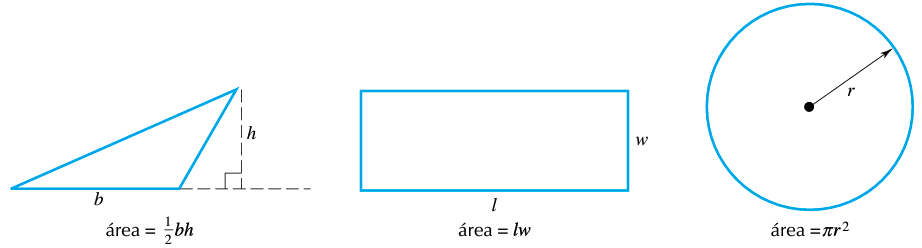
\includegraphics[width=.8\textwidth]{pics/areas-simples.png}}

En este capítulo veremos cómo calcular el área de figuras más generales. Comenzaremos con el cálculo del área que queda delimitada de la siguiente manera:

\noindent
\begin{minipage}{.5\textwidth}
  \begin{itemize}
  \item Por debajo, por el eje $x$;
  \item Por encima, por la gráfica de $y=f(x)$;
  \item A la izquierda por la recta $x=a$; 
  \item A la derecha por la recta $x=b$.
\end{itemize}
\end{minipage}
\begin{minipage}{.5\textwidth}
  \centering
  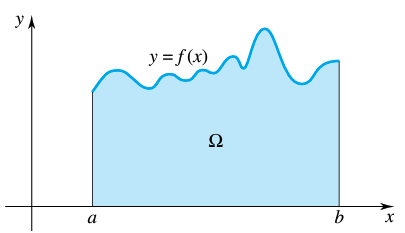
\includegraphics[width=.9\textwidth]{pics/area-bajo-curva.png}
\end{minipage}

\noindent
\begin{minipage}{.5\textwidth}
  Consideramos ahora una subdivisión del intervalo $[a,b]$ en un número finito de subintervalos que no se solapan:
  \[
  [x_0,x_1],\ [x_1,x_2],\dots,\ [x_{n-1},x_n]
  \]
  con $\D a=x_0<x_1<\dots<x_n=b$.

  Observamos que el área de la región $\Omega$ es lo mismo que la suma de las áreas de las regiones $\Omega_i$.
\end{minipage}
\begin{minipage}{.5\textwidth}
  \centering
  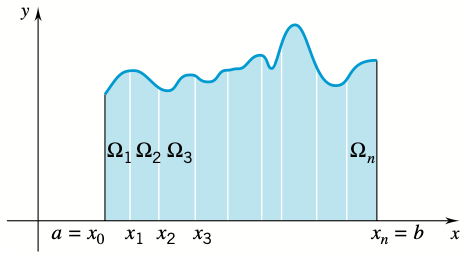
\includegraphics[width=.9\textwidth]{pics/area-bajo-curva-particionada.png}
\end{minipage}

Podemos aproximar el área total de $\Omega$ aproximando el área de cada una de las subregiones $\Omega_i$ y sumando los resultados.
Definimos, para cada $i=1,2,\dots,n$ las siguientes cantidades:
\[ 
  m_i = \min_{x\in [x_{i-1},x_i]}f(x)=\min_{[x_{i-1},x_i]}f,
  \qquad
  M_i = \max_{x\in [x_{i-1},x_i]}f(x)=\max_{[x_{i-1},x_i]}f.
\]
Luego, si $r_i = [x_{i-1},x_i]\times [0,m_i]$ y $R_i = [x_{i-1},x_i]\times [0,M_i]$, resulta que
\[
r_i \subset \Omega_i \subset R_i
\quad\text{y entonces}\quad
\area(r_i)\le \area(\Omega_i) \le \area(R_i).
\]

\centerline{
  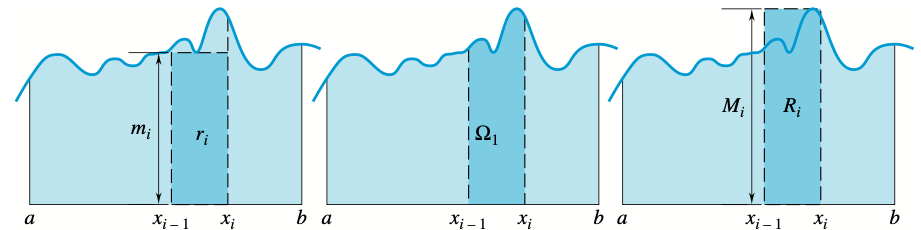
\includegraphics[width=.9\textwidth]{pics/area-omega-i.png}
}

Dado que el área de un rectángulo es el producto de la base por la altura, obtenemos
\[
m_i\, (x_i-x_i-1)
\le \area(\Omega_i) \le
M_i\, (x_i-x_i-1),
\qquad\text{para $i=1,2,\dots,n$}.
\]
Definiendo $\Delta x_i=x_i-x_{i-1}$ tenemos que 
\[
m_i\, \Delta x_i
\le \area(\Omega_i) \le
M_i\, \Delta x_i,
\qquad\text{para $i=1,2,\dots,n$}.
\]
Sumando, obtenemos
\begin{equation}
  \label{eq:L<I<U}
m_1 \Delta x_1 + m_2 \Delta x_2 + \dots + m_n \Delta x_N
\le \area(\Omega_i) \le
M_1 \Delta x_1 + M_2 \Delta x_2 + \dots + M_n \Delta x_N.
\end{equation}
La suma $m_1 \Delta x_1 + m_2 \Delta x_2 + \dots + m_n \Delta x_N$ es una \emph{suma inferior de $f$} 
y la suma $M_1 \Delta x_1 + M_2 \Delta x_2 + \dots + M_n \Delta x_N$ es una \emph{suma superior de $f$}.

\centerline{
  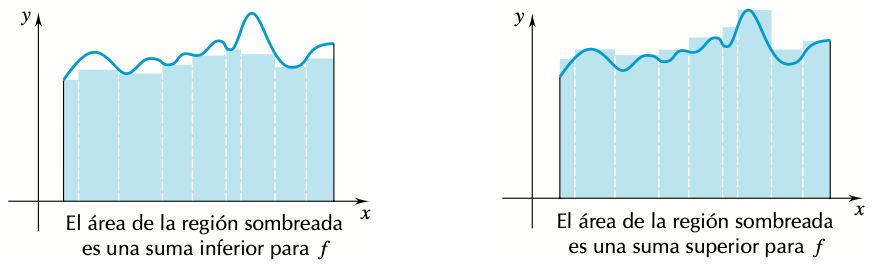
\includegraphics[width=.9\textwidth]{pics/sumas-superiores-inferiores.png}
}

La desigualdad~\eqref{eq:L<I<U} nos dice que para que un número pueda ser candidato al título de \emph{área de $\Omega$}, tal número ha de ser mayor o igual que cualquier suma inferior de $f$ y menor o igual que cualquier suma superior de $f$. Puede demostrarse, aunque no lo veremos aquí, que si $f$ es una función continua en $[a,b]$ entonces existe un número y sólo uno que cumple estas condiciones. A tal número lo llamaremos \emph{área de $\Omega$}.

\subsection*{Integral definida}

El procedimiento seguido para resolver el problema de área se llama \emph{integración} y el resultado final de este procedimiento se denomina \emph{integral definida}. A continuación estableceremos estas nociones con más precisión.

\begin{definition}
  Llamaremos \emph{partición} del intervalo cerrado $[a,b]$ a todo subconjunto finito de $[a,b]$ que contenga a los extremos. Es conveniente identificar los elementos de la partición con un índice acorde al orden narural. Así, cuando escribimos que 
  \[
  P=\{x_0,x_1, \dots ,x_n\} \text{ es una partición de $[a,b]$},
  \]
  entendemos que $\D a=x_0<x_1<\dots<x_n=b$.
\end{definition}

Supongamos ahora que $f$ es una función continua sobre $[a,b]$. En cada subintervalo $[x_{i-1},x_i]$ la función $f$ toma entonces un valor máximo $M_i$ y un mínimo $m_i$. Definimos entonces:

\begin{definition}
  Sea $f$ una función continua sobre $[a,b]$ y sea $P=\{a=x_0<x_1<\dots<x_n=b\}$ una partición de $[a,b]$. Luego definimos, para cada $i=1,2,\dots,n$:
  \[ 
    m_i = \min_{[x_{i-1},x_i]}f,
    \qquad
    M_i = \max_{[x_{i-1},x_i]}f.
  \]
  El número 
  \[
  L(P,f)= m_1 \Delta x_1 + m_2 \Delta x_2 + \dots + m_n \Delta x_N 
  = \sum_{i=1}^n m_i \Delta x_i,
  \]
  se denomina
  \emph{suma inferior de $f$ correspondiente a la partición $P$};
  y el número 
  \[
  U(P,f)= M_1 \Delta x_1 + M_2 \Delta x_2 + \dots + M_n \Delta x_N
  = \sum_{i=1}^n M_i \Delta x_i,
  \]
  se denomina \emph{suma superior de $f$ correspondiente a la partición $P$}.
\end{definition}

\begin{theorem}
  Si $f$ es una función continua en $[a,b]$ existe un único número $I$ que satisface la desigualdad 
  \[
  L(P,f)\le I\le U(P,f),
  \qquad\text{para toda partición $P$ de $[a,b]$}
  \]
\end{theorem}

\begin{proof}
  La demostración de este teorema queda fuera del alcance de este apunte, y será discutida en las clases de Coloquio de Demostraciones.
\end{proof}

A partir de este último teorema llegamos a la definición principal de esta sección:

\begin{definition}[Integral definida]
  Sea $f$ una función continua en $[a,b]$. El único número $I$ que satisface 
  \[
    L(P,f)\le I\le U(P,f),
    \qquad\text{para toda partición $P$ de $[a,b]$}
  \]
  se llama \emph{integral definida} (o simplemente \emph{integral}) de $f$ entre $a$ y $b$ y se designa por
  \[
  \int_a^b f(x)\dx.
  \]
\end{definition}

El símbolo $\int$ fue introducido por Leibniz y se llama \emph{signo integral}. En realidad es una \emph{S} (de \emph{suma}) estirada. Los números $a$ y $b$ se denominan \emph{límites de integración} ($a$ es el límite inferior y $b$ el límite superior). La función a integrar se llama \emph{integrando}. En algunos libros suele escribirse más brevemente $\int_a^b f$, omitiendo la variable $x$.

En la expresión $\int_a^b f(x)\dx$ la variable $x$ es una \emph{variable muda}. Esto quiere decir que puede ser sustituida por cualquier otra letra no utilizada hasta el momento. Así:
\[
\int_a^b f(x)\, dx
= \int_a^b f(t)\, dt
= \int_a^b f(u)\, du
= \int_a^b f(z)\, dz.
\]

En la introducción a este capítulo comenzamos con una aplicación inmediata de la integral definida:
Si $f$ es no negativa en $[a,b]$, entonces
\[
A = \int_a^b f(x)\dx
\]
da como resultado el área debajo de la gráfica de $f$.
Volveremos más adelante sobre esta aplicación.
Ahora veamos algunos ejemplos sencillos que nos ayudarán a comprender la definición.

\begin{example}
  Si $f(x)=c$, una constante, para todo $x\in[a,b]$, ?`cuánto vale $\int_a^b f(x)\dx$?

  Veamos, si $P=\{a=x_0<x_1<\dots<x_n=b\}$ es una partición de $[a,b]$, tenemos que 
\[ 
    m_i = \min_{[x_{i-1},x_i]}f = c
    \qquad
    M_i = \max_{[x_{i-1},x_i]}f = c;
  \]
  por lo que 
  \[
  L(P,f)
  = \sum_{i=1}^n m_i \Delta x_i
  = \sum_{i=1}^n c \Delta x_i
  = c \sum_{i=1}^n \Delta x_i
  = c (b-a)
  \]
  y 
  \[
  U(P,f)
  = \sum_{i=1}^n M_i \Delta x_i
  = \sum_{i=1}^n c \Delta x_i
  = c \sum_{i=1}^n \Delta x_i
  = c (b-a).
  \]
  Luego, 
  \[
    L(P,f)\le c(b-a)\le U(P,f),
    \qquad\text{para toda partición $P$ de $[a,b]$},
  \]
  y concluimos que 
  \[
  \int_a^b f(x)\dx = \int_a^b c \dx = c (b-a).
  \]

  Como ejemplos concretos:
  \begin{align*}
    \int_{-1}^1 3 \dx = 3 \big(1 - (-1)\big) = 3 \cdot 2 = 6;
    % \qquad\text{y}
    \\
    \int_{4}^{10} -3 \dx = -2 \big(10 - 4\big) = -2 \cdot 6 = -12.
  \end{align*}
\end{example}

\begin{example}
  Nos proponemos estudiar ahora la integral de la función $f(x)=x$, es decir $\int_a^b x\dx$.
  Veamos, si $P=\{a=x_0<x_1<\dots<x_n=b\}$ es una partición de $[a,b]$, tenemos que 
  \[ 
      m_i = \min_{[x_{i-1},x_i]}f = x_{i-1}
      \qquad
      M_i = \max_{[x_{i-1},x_i]}f = x_i;
    \]
    por lo que 
    \[
    L(P,f)
    = \sum_{i=1}^n m_i \Delta x_i
    = \sum_{i=1}^n x_{i-1} (x_{i}-x_{i-1})
    \]
    y 
    \[
    U(P,f)
    = \sum_{i=1}^n M_i \Delta x_i
    = \sum_{i=1}^n x_{i} (x_{i}-x_{i-1}).
    \]
    Observamos que para cada índice $i=1,2,\dots,n$, 
    \[
    x_{i-1}\le \frac12 (x_i+x_{i-1})\le x_i.
    \]
    Luego, multiplicando por $\Delta x_i = x_i-x_{i-1}>0$, tenemos que
    \[
    x_{i-1} \Delta x_i 
    \le \frac12 (x_i+x_{i-1})(x_i-x_{i-1}) 
    = \frac12 (x_i^2-x_{i-1}^2) = 
    \le x_i \Delta x_i.
    \]
    Sumando para $i$ de $1$ a $n$ obtenemos
    \[
    L(P,f) \le \sum_{i=1}^n \frac12 (x_i^2-x_{i-1}^2) \le U(P,f).
    \]
    Pero 
    \begin{align*}
      \sum_{i=1}^n \frac12 (x_i^2-x_{i-1}^2)
      &= \frac12 \Big[ (x_1^2-x_0^2) + (x_2^2-x_1^2) + \dots + (x_n^2-x_{n-1}^2)  \Big]
      \\
      &= \frac12 \big(x_n^2-x_0^2\big)
      = \frac12 \big(b^2-a^2\big).
    \end{align*}
    Luego, 
    \[
      L(P,f)\le \frac12 \big(b^2-a^2\big) \le U(P,f),
      \qquad\text{para toda partición $P$ de $[a,b]$},
    \]
    y por lo tanto
    \[
    \int_a^b x\dx = \frac12 \big(b^2-a^2\big).
    \]
    Como ejemplos concretos:
    \begin{align*}
      \int_{-1}^1 x \dx = \frac12 \big(3^2 - (-1)^2\big) = \frac12 \cdot 8 = 4;
      % \qquad\text{y}
      \\
      \int_{-2}^{2} x \dx = \frac12 \big(2^2 - (-2)^2\big) = \frac12 \cdot 0 = 0.
    \end{align*}\end{example}



\subsubsection*{Ejercicios de la sección~\getcurrentref{chapter}.\getcurrentref{section}}

\begin{enumerate}
\item 
\end{enumerate}


\section{Propiedades de la integral}


\subsubsection*{Ejercicios de la sección~\getcurrentref{chapter}.\getcurrentref{section}}

\begin{enumerate}
\item 
\end{enumerate}


\section{Integrabilidad de las funciones continuas}


\subsubsection*{Ejercicios de la sección~\getcurrentref{chapter}.\getcurrentref{section}}

\begin{enumerate}
\item 
\end{enumerate}


\section{El teorema fundamental del Cálculo}


\subsubsection*{Ejercicios de la sección~\getcurrentref{chapter}.\getcurrentref{section}}

\begin{enumerate}
\item 
\end{enumerate}


\section{Integrales impropias}


\subsubsection*{Ejercicios de la sección~\getcurrentref{chapter}.\getcurrentref{section}}

\begin{enumerate}
\item 
\end{enumerate}


\section{El método de sustitución}


\subsubsection*{Ejercicios de la sección~\getcurrentref{chapter}.\getcurrentref{section}}

\begin{enumerate}
\item 
\end{enumerate}


\section{El método de integración por partes}


\subsubsection*{Ejercicios de la sección~\getcurrentref{chapter}.\getcurrentref{section}}

\begin{enumerate}
\item 
\end{enumerate}


\section{El método de integración por fracciones simples}


\subsubsection*{Ejercicios de la sección~\getcurrentref{chapter}.\getcurrentref{section}}

\begin{enumerate}
\item 
\end{enumerate}



\subsection*{Ejercicios del capítulo~\getcurrentref{chapter}}



